\documentclass[a4paper, 12pt]{report}
\usepackage[T2A]{fontenc} 
\usepackage[utf8]{inputenc}
\usepackage[english,russian]{babel} 
\usepackage{amsmath,amsfonts,amssymb,amsthm,mathtools}
\usepackage[left=2cm,right=2cm,top=2cm,bottom=2cm,bindingoffset=0cm]{geometry}
\usepackage{graphicx}
\usepackage[linesnumbered,boxed]{algorithm2e}
\usepackage{verbatim}
\usepackage{booktabs}

\newenvironment{Proof} 
{\par\noindent{$\blacklozenge$}}
{\hfill$\scriptstyle\boxtimes$} 

\newenvironment{example} 
{\par\noindent{\textsc{\textbf{Пример}.}}} 
{\hfill$\scriptstyle\Box$} 

\newtheorem*{theorem}{Теорема} 
\newtheorem*{corollary}{Следствие}
\newtheorem*{lemma}{Лемма}

\newcommand{\RNumb}[1]{\uppercase\expandafter{\romannumeral #1\relax}}
\newcommand{\Rm}{\mathbb{R}}
\newcommand{\Cm}{\mathbb{C}}
\newcommand{\I}{\mathbb{I}}
\newcommand{\N}{\mathbb{N}}
\newcommand{\Z}{\mathbb{Z}}
\newcommand{\Q}{\mathbb{Q}}

\title{\textbf{\Huge{Методы вычислений}}\\Лабораторная работа 1\\Численные методы решения нелинейных уравнений\\Выполнила Николаева Ксения, 9 группа}
\date{} 

\begin{document}
    \maketitle

    \textbf{\Huge{Постановка задачи}}\\\\
Дано нелинейное уравнение:
\[
    f(x) = x e^x + x^2 - 1 = 0, \quad x < 0
\]
Необходимо:
\begin{itemize}
    \item Графически отделить корень уравнения $f(x) = 0$.
    \item Сузить отрезок отделенного корня методом дихотомии с точностью $varepsilon = 10^{-2}$.
    \item Найти решение уравнения $f(x) = 0$ с точностью $varepsilon = 10^{-7}$ методами:
    \begin{itemize}
        \item Методом Ньютона с постоянной производной,
        \item Методом Ньютона,
        \item Методом секущих.
    \end{itemize}
    \item Провести сравнительный анализ полученных результатов.
\end{itemize}

\newpage
\textbf{\Huge{Результаты работы}}\\\\

\begin{figure}
    \centering
    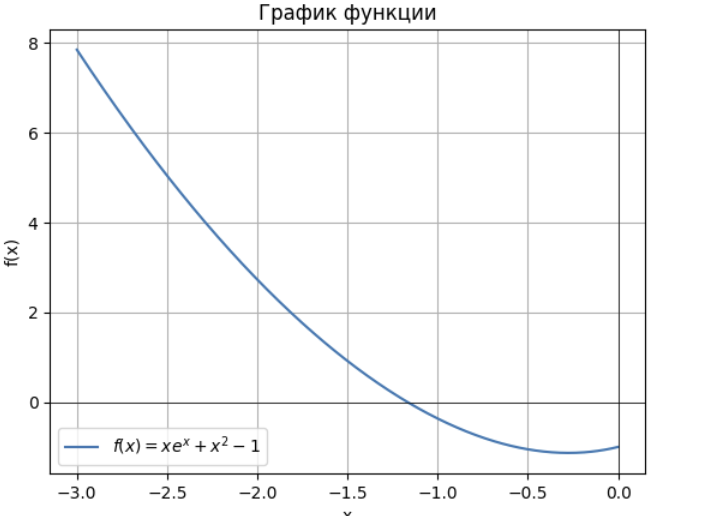
\includegraphics[width=0.7\linewidth]{image.png}
    \caption{График функции, отделенный отрезок [-2, -1]}
    \label{fig:enter-label}
\end{figure}

\textbf{Метод дихотомии}\\
Метод дихотомии используется для нахождения корня функции на отрезке \([a, b]\). Он основан на повторном делении отрезка пополам. Если функция \( f(x) \) имеет разные знаки на концах отрезка, то на одном из подотрезков будет корень. Алгоритм продолжает делить отрезок до тех пор, пока длина отрезка не станет меньше заданного порога \(\epsilon\).

\begin{verbatim}
def dichotomy_method(a, b, epsilon=1e-2):
    k = 0
    while (b - a) / 2 > epsilon:
        c = (a + b) / 2
        if f(c) == 0:
            return c, results
        elif f(a) * f(c) < 0:
            b = c
        else:
            a = c
        k += 1
    return (a + b) / 2, results
\end{verbatim}

\textbf{Корень по методу дихотомии:} $x \approx -1.1640625$
\begin{table}[h]
    \centering
    \begin{tabular}{cccccc}
        \toprule
        $k$ & $a_k$ & $b_k$ & $f(a_k)$ & $f(b_k)$ & $b_k - a_k$ \\
        \midrule
        0 & -2.000000 & -1.00000 & 2.729329 & -0.367879 & 1.000000 \\
        1 & -1.500000 & -1.00000 & 0.915305 & -0.367879 & 0.500000 \\
        2 & -1.250000 & -1.00000 & 0.204369 & -0.367879 & 0.250000 \\
        3 & -1.250000 & -1.12500 & 0.204369 & -0.099609 & 0.125000 \\
        4 & -1.187500 & -1.12500 & 0.047989 & -0.099609 & 0.062500 \\
        5 & -1.187500 & -1.15625 & 0.047989 & -0.026916 & 0.031250 \\
        6 & -1.171875 & -1.15625 & 0.010261 & -0.026916 & 0.015625 \\
        \bottomrule
    \end{tabular}
    \caption{Результаты метода дихотомии}
\end{table}

\textbf{Метод Ньютона с постоянной производной}\\
Метод Ньютона с постоянной производной используется для нахождения корня функции, при этом предполагается, что производная функции \( f'(x) \) постоянна. Алгоритм итеративно улучшает приближение корня, используя формулу \( x_{n+1} = x_n - \frac{f(x_n)}{f'(x_n)} \).
\begin{verbatim}
    def newton_method_constant_derivative(x0, epsilon=1e-7):
    k = 0
    x = x0
    while abs(f(x)) > epsilon:
        x = x - f(x) / f_prime(x0)
        k += 1
    return x
\end{verbatim}

\textbf{Метод Ньютона}\\
Метод Ньютона используется для нахождения корня функции, используя ее производную. Начальное приближение \(x_0\) подставляется в формулу итерации, и на каждом шаге улучшение приближения вычисляется с учетом текущей производной функции.
\begin{verbatim}
    def newton_method(x0, epsilon=1e-7):
    k = 0
    x = x0
    while abs(f(x)) > epsilon:
        x = x - f(x) / f_prime(x)
        k += 1
    return x
\end{verbatim}

\textbf{Метод секущих}\\
Метод секущих является итерационным методом нахождения корней функции. Он не требует вычисления производной, вместо этого используется секущая линия, проходящая через две последние точки. На каждом шаге новые значения для \(x_0\) и \(x_1\) обновляются в зависимости от значения функции в этих точках.
\begin{verbatim}
    def secant_method(x0, x1, epsilon=1e-7):
    k = 0
    while abs(f(x1)) > epsilon:
        x2 = x1 - f(x1) * (x1 - x0) / (f(x1) - f(x0))
        x0, x1 = x1, x2
        k += 1
    return x1
\end{verbatim}


\begin{table}[h]
    \centering
    \small
    \begin{tabular}{|c|c|c|c|}
        \hline
        $k$ & Метод Ньютона с постоянной производной & Метод Ньютона & Метод секущих \\
        \hline
        0 & -1.167591 & -1.167591 & -1.118778 \\
        \hline
        1 & -1.167586 & -1.167586 & -1.171989 \\
        \hline
        2 & — & — & -1.167481 \\
        \hline
        3 & — & — & -1.167585 \\
        \hline
        4 & — & — & -1.167586 \\
        \hline
        \hline
        $|x_k - x_{k-1}|$ & $1.407421 \times 10^{-5}$ & $1.407421 \times 10^{-5}$ & $1.138174 \times 10^{-1}$ \\
        \hline
        $|x_k - x_{k-1}|$ & $4.713562 \times 10^{-8}$ & $3.925593 \times 10^{-11}$ & $1.053443 \times 10^{-2}$ \\
        \hline
        — & — & — & $2.489199 \times 10^{-4}$ \\
        \hline
        — & — & — & $5.173854 \times 10^{-7}$ \\
        \hline
        — & — & — & $2.552580 \times 10^{-11}$ \\
        \hline
    \end{tabular}
    \caption{Сводные данные по результатам работы методов}
\end{table}


\newpage
\textbf{\Huge{Выводы}}\\\\
$\bullet$ Метод дихотомии потребовал больше всего итераций, но гарантированно сужал интервал.\\
$\bullet$ Метод Ньютона и его модификация с постоянной производной показали быстрый сход, но требуют знания производной.\\
$\bullet$ Метод секущих сошелся за 5 итераций, не требуя производной, что делает его эффективным.\\
$\bullet$ Все методы показали сход к корню $x \approx -1.1675855268$, что подтверждает их корректность и сходимость.

\newpage
\textbf{\Huge{Листинг программы}}\\\\

\begin{verbatim}
import numpy as np
import matplotlib.pyplot as plt

# Определяем функцию
def f(x):
    return x * np.exp(x) + x**2 - 1

# Построение графика
x_vals = np.linspace(-3, 0, 400)
y_vals = f(x_vals)

plt.plot(x_vals, y_vals, label=r'$f(x) = x e^x + x^2 - 1$')
plt.axhline(0, color='black',linewidth=0.5)
plt.axvline(0, color='black',linewidth=0.5)
plt.title('График функции')
plt.xlabel('x')
plt.ylabel('f(x)')
plt.grid(True)
plt.legend()
plt.show()


# Метод дихотомии
def dichotomy_method(a, b, epsilon=1e-2):
    k = 0
    results = []
    while (b - a) / 2 > epsilon:
        c = (a + b) / 2
        results.append([k, a, b, f(a), f(b), b - a])
        if f(c) == 0:
            return c, results
        elif f(a) * f(c) < 0:
            b = c
        else:
            a = c
        k += 1
    results.append([k, a, b, f(a), f(b), b - a])
    return (a + b) / 2, results

# Отрезок отделенного корня
a, b = -2, -1  # Начальный интервал
root_dichotomy, dichotomy_results = dichotomy_method(a, b, epsilon=1e-2)
print(f"Корень по методу дихотомии: {root_dichotomy}")

# Производная функции
def f_prime(x):
    return np.exp(x) * (x + 1) + 2 * x

# Метод Ньютона с постоянной производной
def newton_method_constant_derivative(x0, epsilon=1e-7):
    k = 0
    x = x0
    results = []
    while abs(f(x)) > epsilon:
        x = x - f(x) / f_prime(x0)
        results.append([k, x, abs(f(x))])
        k += 1
    return x, results

# Корень по методу Ньютона с постоянной производной
root_newton_constant, newton_constant_results = newton_method_constant_derivative(root_dichotomy, epsilon=1e-7)
print(f"Корень по методу Ньютона (с постоянной производной): {root_newton_constant}")

# Метод Ньютона
def newton_method(x0, epsilon=1e-7):
    k = 0
    x = x0
    results = []
    while abs(f(x)) > epsilon:
        x = x - f(x) / f_prime(x)
        results.append([k, x, abs(f(x))])
        k += 1
    return x, results

# Корень по методу Ньютона
root_newton, newton_results = newton_method(root_dichotomy, epsilon=1e-7)
print(f"Корень по методу Ньютона: {root_newton}")

# Метод секущих
def secant_method(x0, x1, epsilon=1e-7):
    k = 0
    results = []
    while abs(f(x1)) > epsilon:
        x2 = x1 - f(x1) * (x1 - x0) / (f(x1) - f(x0))
        results.append([k, x2, abs(f(x2))])
        x0, x1 = x1, x2
        k += 1
    return x1, results

\end{verbatim}

\end{document}


